
\chapter{\IfLanguageName{dutch}{Praktische uitvoering van nummerplaatdetectie op UGent}{Implementation of ANPR at UGent}}
\label{ch:praktischeUitvoering}
In dit hoofdstuk zal er onderzocht worden of nummerplaatdetectie degelijke resultaten kan leveren op de Campus Sterre en Campus Coupure van UGent. Hiervoor zullen handmatig foto's genomen worden van wagens die de parking willen verlaten met de Pi-NoIR cam. Hierna wordt er gecontroleerd of OpenANPR wel degelijk correcte resultaten levert op de genomen foto's.


\section{Hardware en software}
In dit onderdeel worden de maatregelingen uit hoofdstuk 5 toegepast op de case van UGent.

\subsection{Camera}
Als camera zal gebruik gemaakt worden van de PiNoIR-Cam. Deze camera is een standaard extensie voor de Raspberry-PI die geen infrarood filtering heeft staan. Standaard wordt infrarood uit afbeeldingen gefilterd omdat deze een ongewenst bijproduct zijn op foto's. De PiNoIR camera filtert geen infrarood uit de afbeeldingen en maken het dus mogelijk om te gebruiken voor infrarood detectie.

\paragraph{Cameraplaatsing}
Voor de plaatsing van de camera's wordt er gewenst zo veel mogelijk kosten te besparen en wordt er liever niet geopteerd voor een aparte paal voor de ANPR-camera. Daarom zal als fotopunt de metalen constructie van de hefboom gekozen worden. De camera zal hier zo hoog mogelijk aan worden gehangen zodat deze zo min mogelijk interferentie heeft van de koplampen van de auto's.

\begin{figure}[h!]
	\centering
	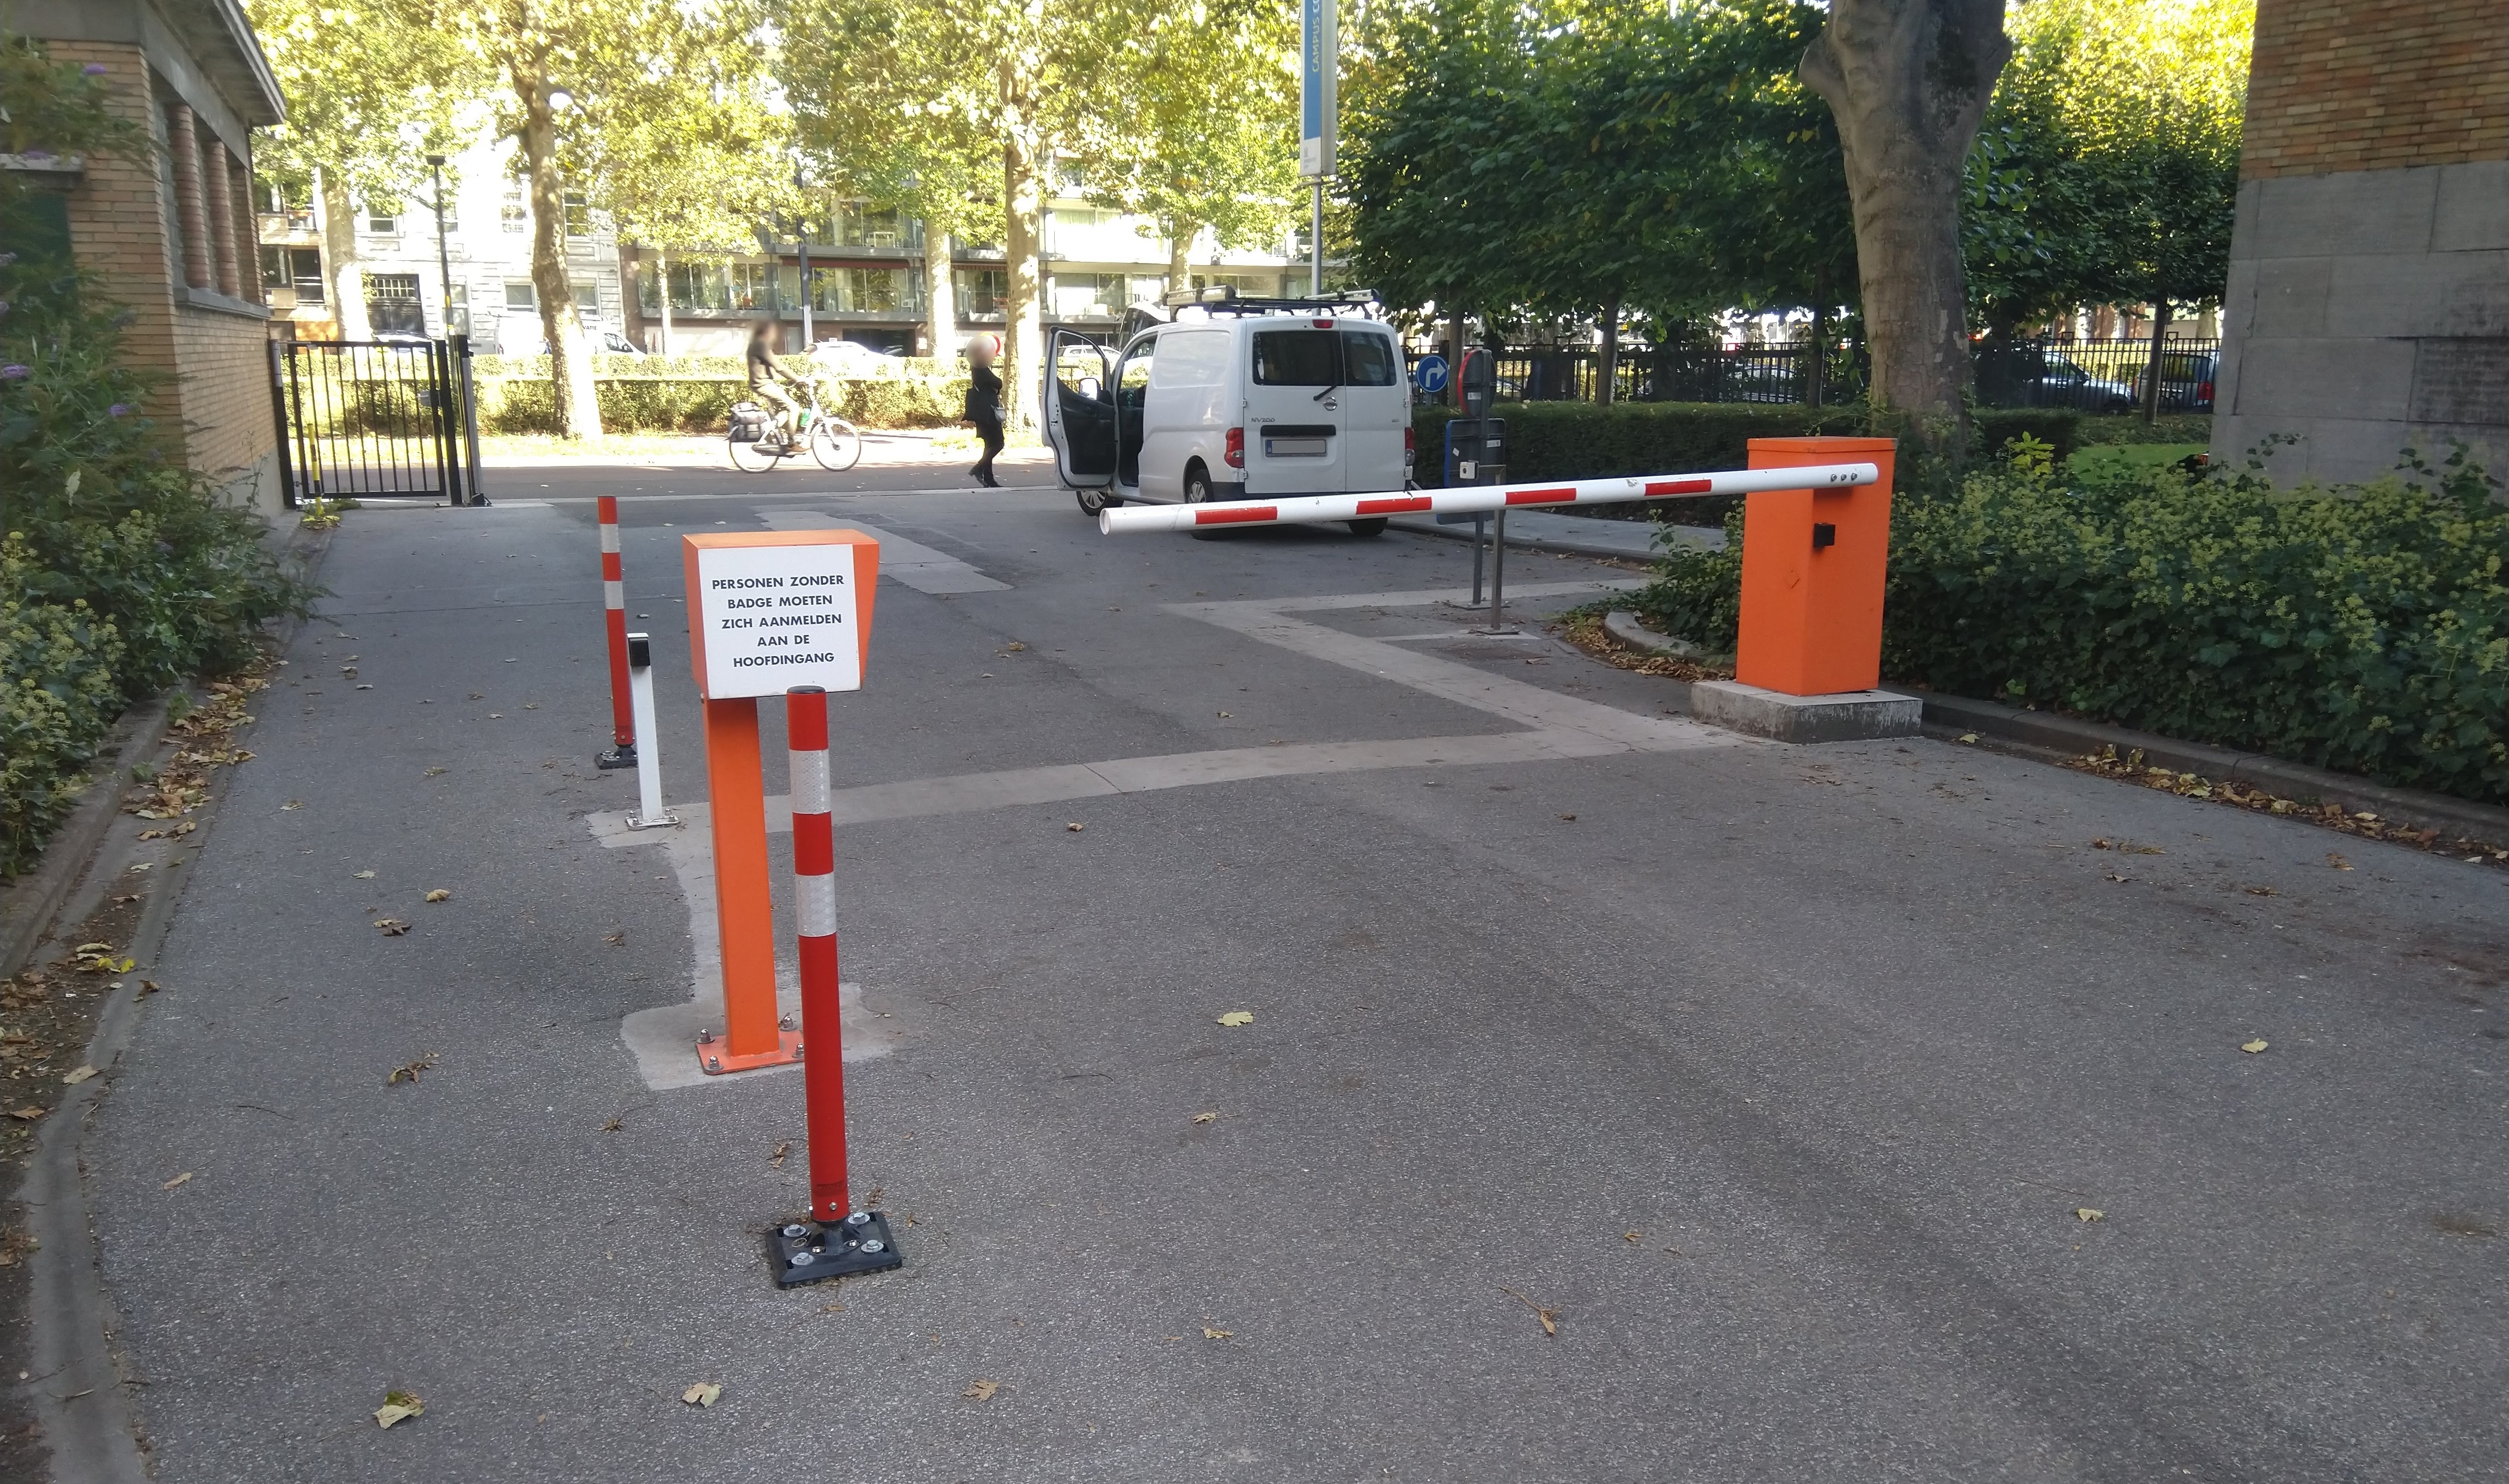
\includegraphics[width=\linewidth]{img/uitgang-coupure.jpg}
	\caption{Uitgang met tokens aan UGent campus Coupure}
\end{figure}

\paragraph{Cameraconfiguratie}
De voorgaande camerainstellingen zullen zo correct mogelijk op de PiNoIR camera worden ingesteld.
TODO: Beste raspistill commando instellingen vinden.

\section{Dataset collectie}
Om een correcte dataset te bekomen zal er op de parking van UGent zelf data verzameld worden aan de corresponderende ingangen. Er zijn geen cijfers beschikbaar over welke uitgangen meer gebruikt worden, daarom zullen de cijfers aan iedere ingang apart verwerkt worden.

Voor iedere uitgang (4) zullen een honderd foto's genomen worden van voertuigen die de parking verlaten in verscheidene omstandigheden zoals licht/donker/regen en zal bij iedere foto genoteerd worden welke nummerplaat correct is

\section{Verwerking van gegevens}

Opslitsen data voor dag, nacht, regen en verschillende ingangen/uitgangen.
alpr uitvoeren op alle afbeeldingen en checken of ze correct zijn. Rekening houden met orientatie zodat de publieke weg niet in beeld is.